\documentclass[final]{beamer}
\usepackage[scale=1.24]{beamerposter}
\usepackage{graphicx,booktabs,tabularx}
\usepackage{helvet,tikz}

\usetikzlibrary{arrows,fit,patterns}


\usetheme{confposter}
\setbeamercolor{block title}{fg=Maroon,bg=white}
\setbeamercolor{block body}{fg=black,bg=white}
\setbeamercolor{block alerted title}{fg=white,bg=Maroon!70}
\setbeamercolor{block alerted body}{fg=black,bg=Maroon!10}

\newlength{\sepwid}
\newlength{\onecolwid}
\newlength{\twocolwid}
\newlength{\threecolwid}
\setlength{\paperwidth}{48in}
\setlength{\paperheight}{48in}
\setlength{\sepwid}{0.024\paperwidth}
\setlength{\onecolwid}{0.22\paperwidth}
\setlength{\twocolwid}{0.464\paperwidth}
\setlength{\threecolwid}{0.708\paperwidth}
\setlength{\topmargin}{-0.5in}
\newcolumntype{Y}{>{\centering\arraybackslash}X}


\title{Fido: A Universal Robot Control System Using\\Reinforcement Learning with Limited Feedback}
\author{\LARGE Joshua Gruenstein \and Michael Truell}
\institute{\mbox{}}

\begin{document}

\addtobeamertemplate{block end}{}{\vspace*{2ex}}
\addtobeamertemplate{block alerted end}{}{\vspace*{2ex}}
\setlength{\belowcaptionskip}{2ex}
\setlength\belowdisplayshortskip{2ex}

\begin{frame}[t]
\begin{columns}[t]

\begin{column}{\sepwid}\end{column}
\begin{column}{\onecolwid}

	\begin{alertblock}{Control System Objectives}
		Fido was created to fulfill the following goals:
		\begin{itemize}
			\item \textbf{Trainability}: Allow both human and autonomous training and retraining rather than programming
			\item \textbf{Universality}: Run on any robot and perform any task, even without prior knowledge of the host
			\item \textbf{Performance}: Require few learning iterations and low latency for quick and efficient training
		\end{itemize}
		To achieve this we developed a novel machine learning algorithm utilizing wire-fitted Q-Learning with a neural network, a probabilistic action selection model, and history sampling.  The control system could be trained at a rate \textbf{3 times} the industry standard, allowing practicality over traditional pre-programmed control systems.
	\end{alertblock}

	\begin{block}{System Overview}
		\begin{figure}
			\centering
			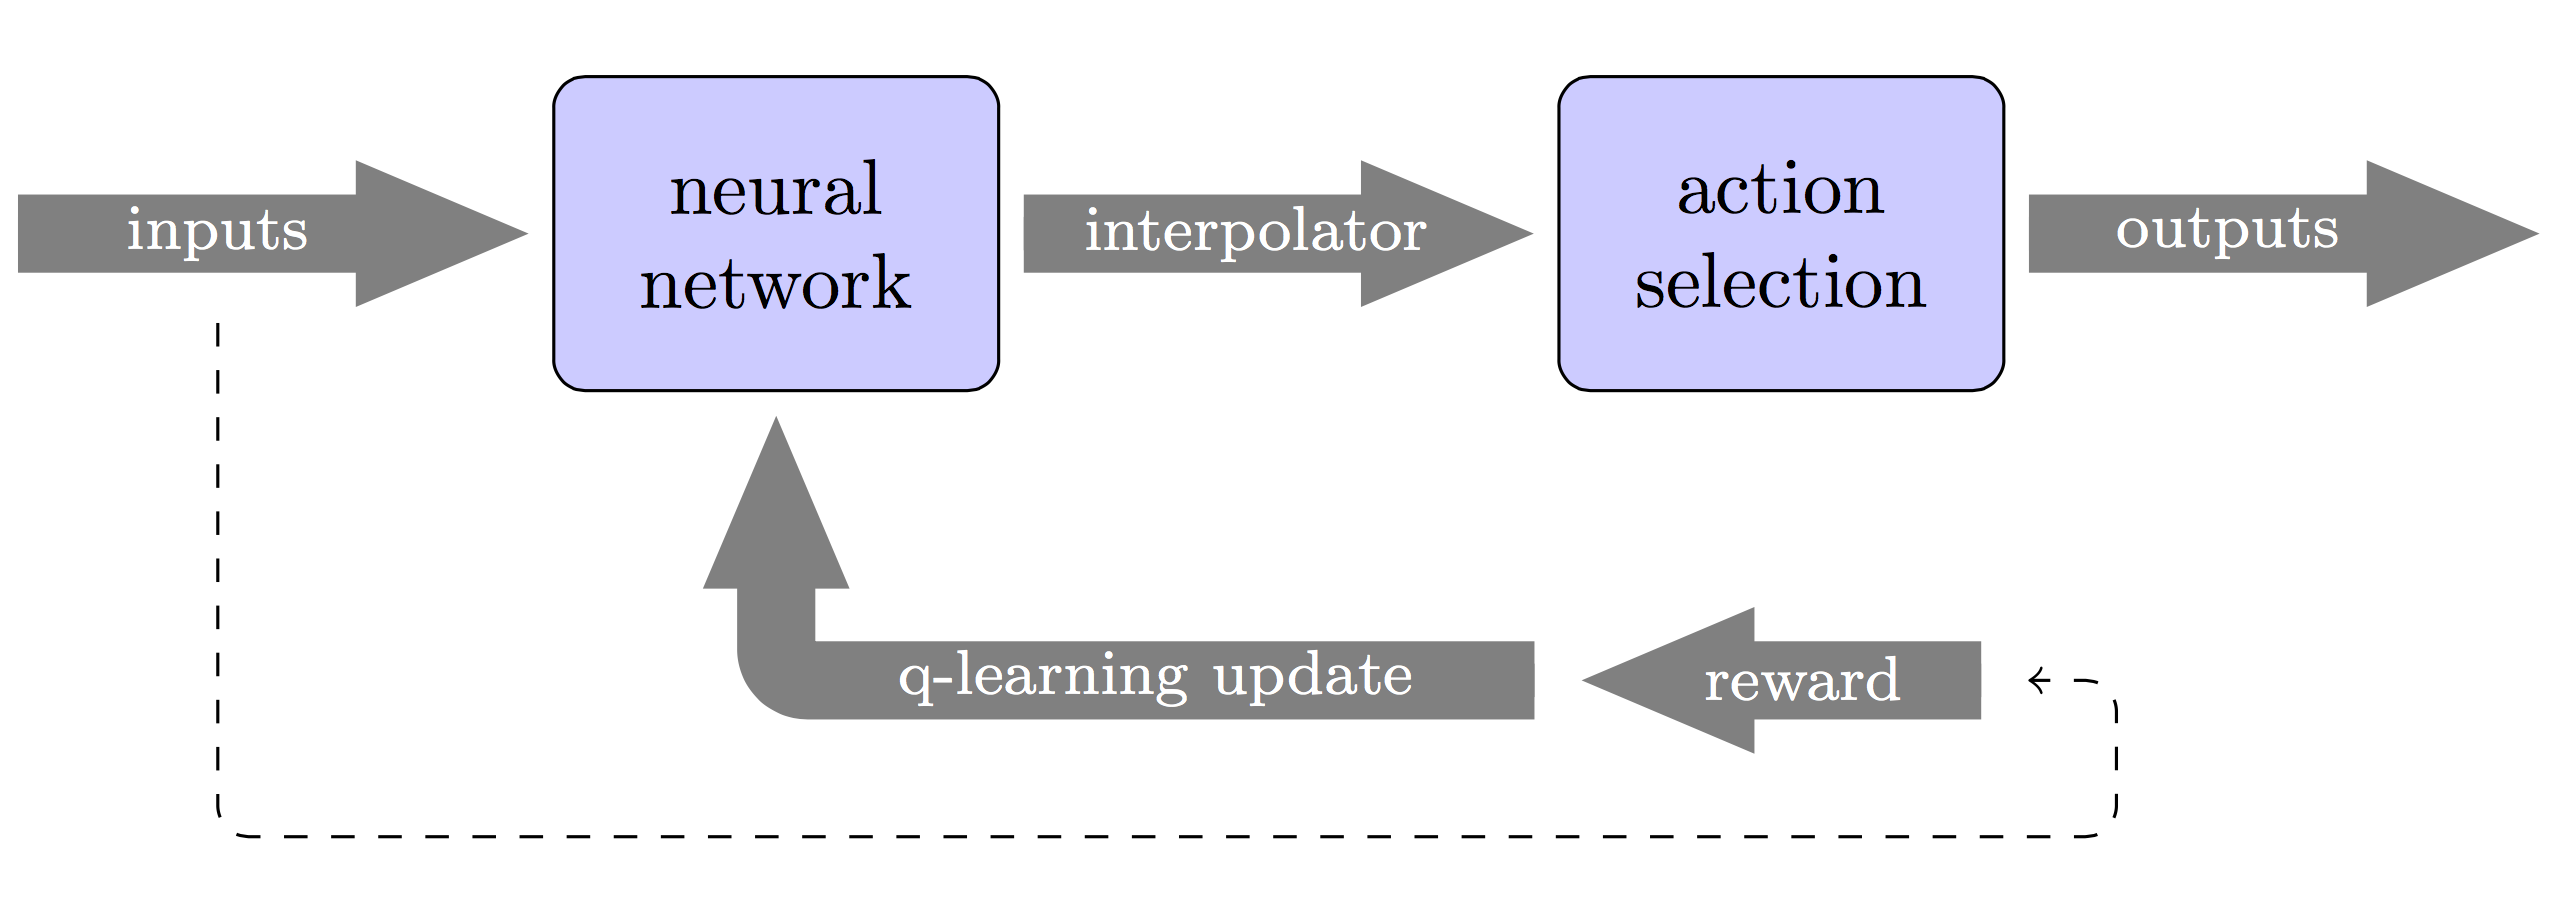
\includegraphics[width=\linewidth]{Figures/diagramRendered.png}
			\caption{Control System Diagram}
		\end{figure}
		\vspace{-1cm}
		From a macro perspective, Fido can be viewed as a ``black box'' system, where a set of inputs (such as sensors) go in and a set of outputs (actions) go out.  Fido's goal is to maximize given reward by altering its behavior.  The system operates through the following steps:

		\begin{enumerate}
			\item Sensor values are fed to a neural network.
			\item The neural network outputs data points, each is an action and its expected reward.
			\item A wire-fitted least squares interpolator creates a continuous function of action to expected reward using these data points.
			\item An action is chosen using an Softmax selection policy that dynamically adjusts Fido's exploration level as its confidence level changes.
			\item After receiving reward, the neural network is trained to output a new set of data points using Adadelta for gradient descent. Dynamic sizing of the neural network and history sampling are employed to improve neural network performance.
		\end{enumerate}
	\end{block}

\end{column}

\begin{column}{\sepwid}\end{column}

\begin{column}{\twocolwid}

\vspace{-1.65cm}

\begin{columns}[t,totalwidth=\twocolwid]

	\begin{column}{\onecolwid}
		\begin{block}{Reinforcement Learning}
			\begin{itemize}
				\item \textbf{Q-Learning:} Develops a function that intakes a state-action pair and outputs expected utility
				\item Problem: the Q-function is ordinarily modeled by storing state-action pairs in a table, but this is impractical for large state spaces
				\begin{itemize}
					\item Solution: use a function approximator instead to model the Q-function: \textbf{Artificial Neural Networks}
				\end{itemize}
				\item Problem: with regular Q-Learning, no relation is made between similar states or actions
				\begin{itemize}
					\item Solution: can be optimized by coupling a wire-fitted interpolator with our neural network (\textbf{Wire-Fitted Q-Learning})
				\end{itemize}

				\item Complete solution: neural network is given sensor values and outputs data points on a graph of possible action vs expected utility, which are interpolated and used to generate a continuous function of action to expected reward.
			\end{itemize}
			\vspace{-1.25cm}
		\end{block}
		\begin{block}{Action Selection}
			\begin{itemize}
				\item Problem: cannot just perform the action with the greatest expected utility: must ``explore'' to be trainable and re-trainable
				\begin{itemize}
					\item Solution: use a Softmax Probability Distribution to select an action
				\end{itemize}
				\item Problem: cannot just hardcode the exploration level, Fido should stop exploring if confident in its actions and explore more if it is being retrained
				\begin{itemize}
					\item Solution: measure confidence using changes in the neural network weight matrix and adjust exploration accordingly
				\end{itemize}
			\end{itemize}
		\end{block}
	\end{column}

	\begin{column}{\onecolwid}\begin{block}{Training}

	\begin{figure}
		\centering
		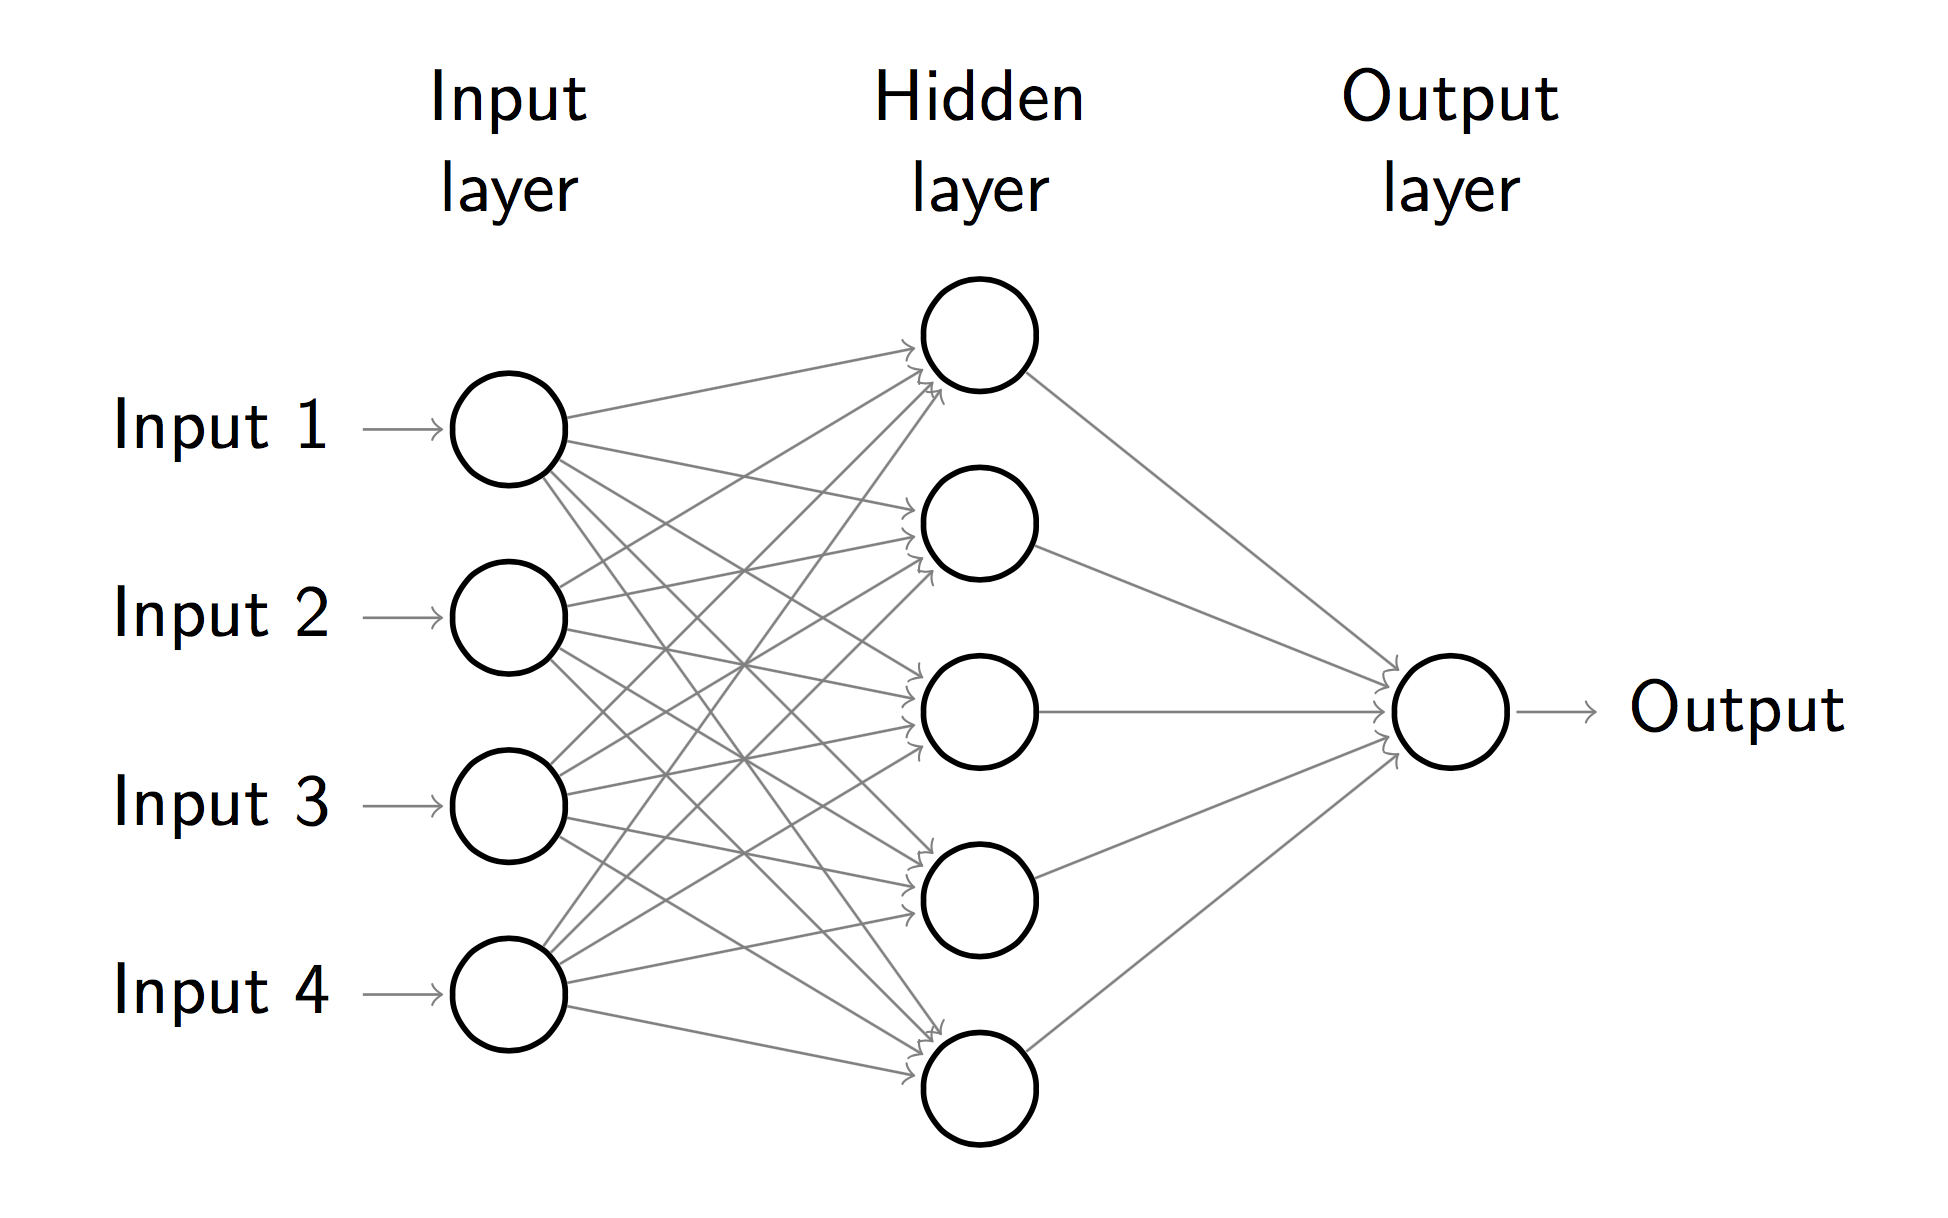
\includegraphics[width=.8\linewidth]{Figures/FeedForwardRendered}
		\caption{Single Output Feed-forward Neural Network}
		\label{fig:feedforward}
	\end{figure}

	\begin{itemize}
		\item Problem: need to update model after receiving reward
		\begin{itemize}
			\item Solution: use Stochastic Gradient Descent to generate a new action to expected reward function for the past state, then train the neural network to output the data points that define this function.
		\end{itemize}
		\item Problem: many neural network training algorithms require a learning rate that depends on the specifics of the task
		\begin{itemize}
			\item Solution: use the new Adadelta training method which dynamically adjusts learning rate, decreases latency, and results in better neural network accuracy
		\end{itemize}
		\item \textbf{Control sequences: } randomly train the neural network on some of Fido's past actions every reward iteration. Give greater weight to newer actions.
		\begin{itemize}
			\item Allows training of action sequences for complex, memory-based tasks
		\end{itemize}
		\item Problem: optimal neural network architecture depends on the task tasks. Ex. larger networks are more suited for complicated tasks.
		\begin{itemize}
			\item Solution: efficiently grow and prune Fido's neural network using neuron sensitivity approximations gathered from fluctuations in the network's weights.
		\end{itemize}
	\end{itemize}

\end{block}\end{column}

\end{columns}


	\begin{block}{Results}
		Results were gathered both from simulation and hardware for a variety of tasks.  Gathered data for each task included the number of learning iterations, or how many pieces of reward it took for Fido to master the task, action selection time, or latency in probabalistic action selection, and training time, or latency in updating Fido's model.
		\begin{table}[ht]
			\centering
			\caption {Fido Results in Simulation} \label{tab:simresults}
			\begin{tabularx}{.9\textwidth}{l||Y|Y|Y}
				\toprule
				Task        & Learning Iterations & Action Selection (ms) & Training Time (ms) \\ \midrule
				Flash       & 6                   & 0.                  & 6               \\
				Float to Point       & 14                  & 1                  & 6               \\
				Drive to Point       & 17                  & 1                  & 11              \\
				Line Following       & 18                                    & 0.               & 2               \\
				Noisy Line Following       & 21                                   & 0.               & 105               \\
				\bottomrule
			\end{tabularx}
		\end{table}
		\vspace{.5cm}

		\begin{table}[ht]
			\centering
			\caption {Fido Results on Thing One} \label{tab:thingoneresults}
			\begin{tabularx}{.9\textwidth}{l||Y|Y|Y}
				\toprule
				Task              & Learning Iterations & Action Selection (ms) & Training Time (ms) \\ \midrule
				Stay Still        & 3                   & 1                    & 43.5                  \\
				Drive to Point    & 18                  & 4                     & 65                  \\
				\bottomrule
			\end{tabularx}
		\end{table}

		\begin{table}[ht]
			\centering
			\caption {Fido Results on Thing Two} \label{tab:thingtworesults}
			\begin{tabularx}{.9\textwidth}{l||Y|Y|Y}
				\toprule
				Task              & Learning Iterations & Action Selection (ms) & Training Time (ms) \\ \midrule
				Drive Straight         & 13                   & 2                    & 30                 \\
				Line Following         & 15                  & 21                    & 95                \\
				Fetch                  & 8                  & 1                     & 70                 \\
				Limping Line Following & 6                   & 20                    & 37                 \\
				\bottomrule
			\end{tabularx}
		\end{table}

	\end{block}

\end{column}

\begin{column}{\sepwid}\end{column}

\begin{column}{\onecolwid}
	\begin{block}{Implementation}
		\setlength\parindent{48pt}
		\indent The Fido control system was programmed in C++, with no external dependencies. Two hardware implementations and a simulator were constructed to test Fido's performance.  The first robot utilized a differential drive system and was powered by an Intel Edison embedded GNU/Linux computing platorm, while the second used a holonomic 3x swedish 90 degree wheel arrangment and ran on a \$5 Raspberry Pi Zero.

		\begin{figure}
			\centering
			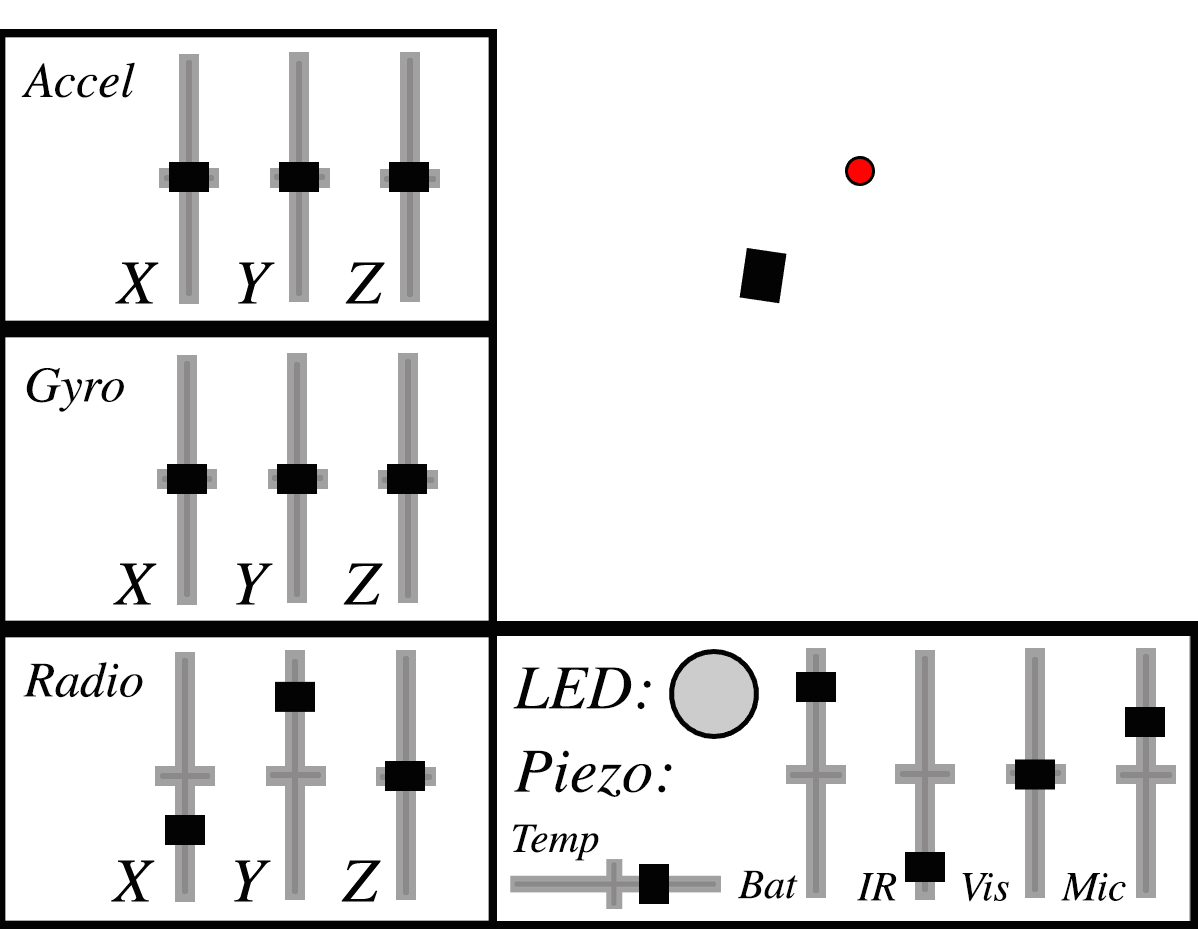
\includegraphics[width=.75\linewidth]{Figures/Screenshot.png}
			\caption{Fido Simulator Graphical User Interface}
		\end{figure}

		\vspace{-0.5in}

		\begin{figure}[ht]
			\centering
			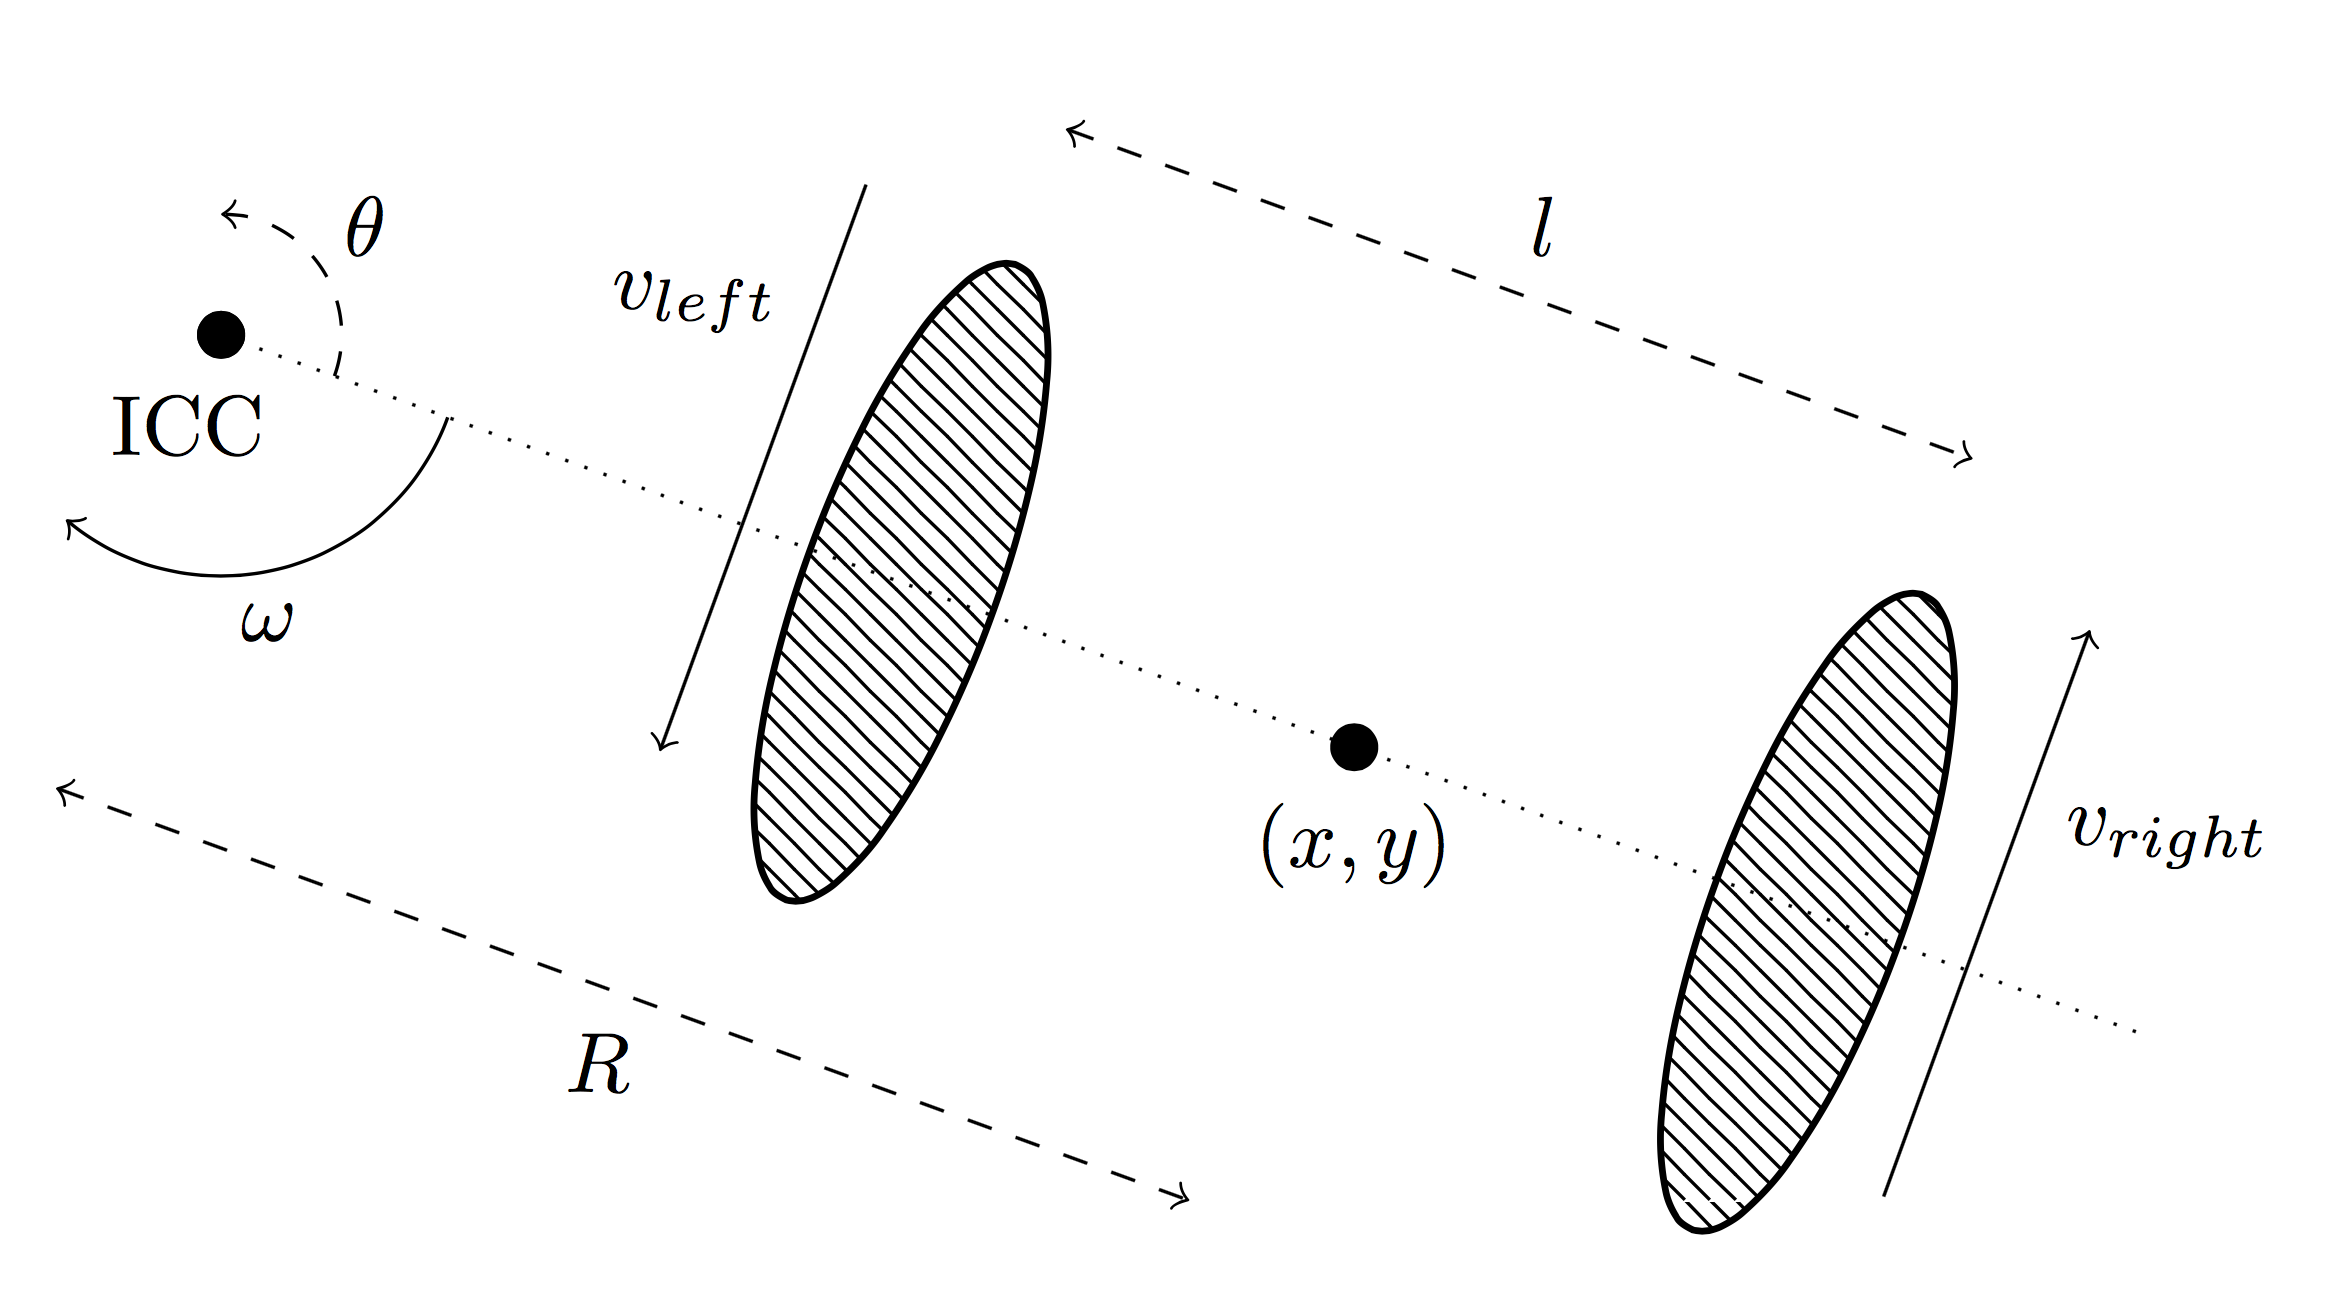
\includegraphics[width=.75\linewidth]{Figures/differentialKinematicsRendered.png}
			\caption{Differential Drive Kinematics}
		\end{figure}

		\vspace{-0.5in}

		\begin{figure}[ht]
			\centering
			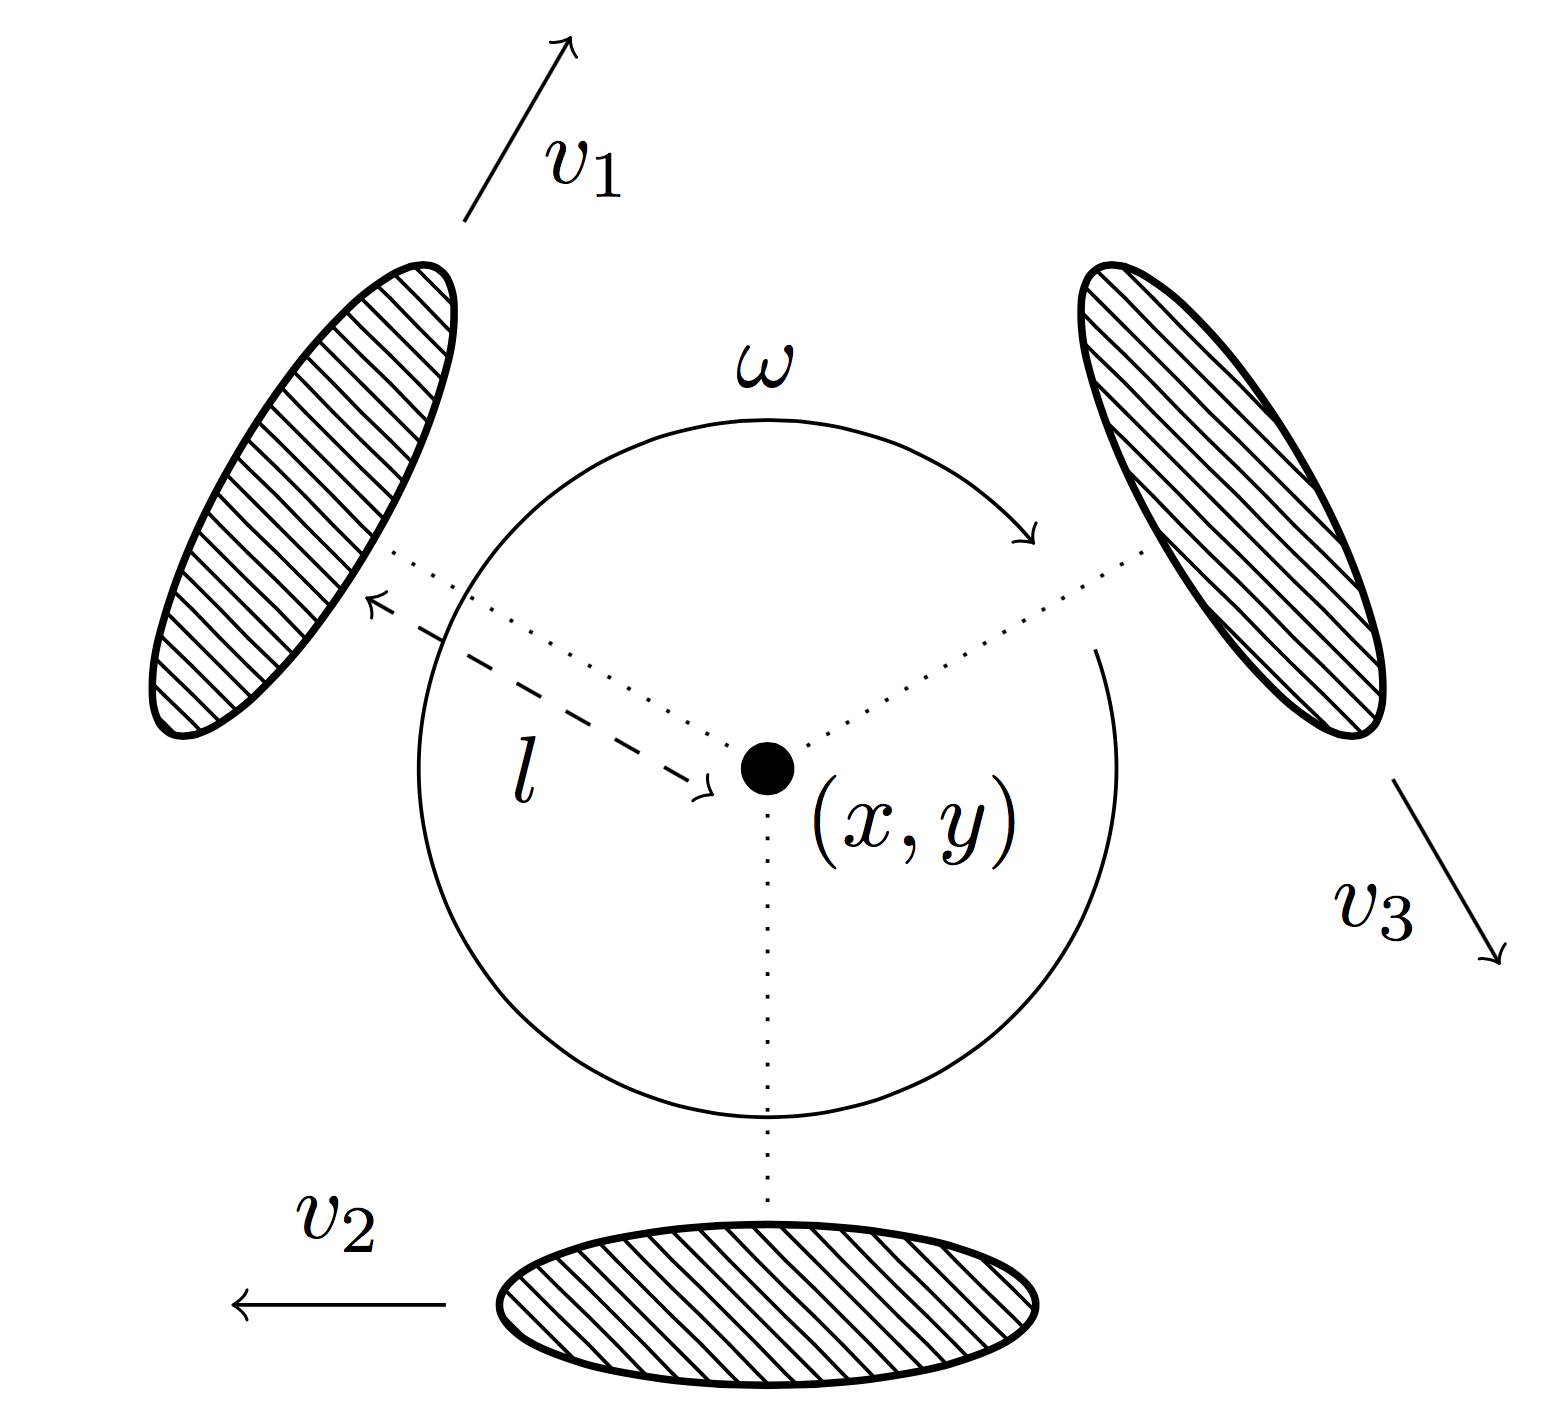
\includegraphics[width=.5\linewidth]{Figures/kiwiKinematicsRendered.png}
			\caption{Holonomic Kiwi Drive Kinematics}
		\end{figure}
	\end{block}

	\begin{block}{Applications}
		Support small businesses, rebuild the military.
	\end{block}

	\begin{block}{Selected References}
		\nocite{*}
		{\fontsize{25}{30}\bibliographystyle{IEEEtran}\bibliography{Poster}\vspace{0.75in}}
	\end{block}

\end{column}

\end{columns}
\end{frame}
\end{document}

%%%%%%%%%%%%%%%%%%%%%%%%%%%%%%%%%%%%%%%%%
% Adapted from "Jacobs Landscape Poster"
% https://teamwork.jacobs-university.de:8443/confluence/display/CoPandBiG/LaTeX+Poster
% License: CC BY-NC-SA 3.0 (http://creativecommons.org/licenses/by-nc-sa/3.0/)
%%%%%%%%%%%%%%%%%%%%%%%%%%%%%%%%%%%%%%%%%
